\subsection{Protocolo de Federated Learning}\label{Protocolo}
El protocolo de Federated Learning que se va a reproducir en este proyecto es una adaptación de lo que proponen los autores de \autocite{bonawitzFederatedLearningScale2019a}. En este protocolo se definen tres fases importantes, la selección de participantes, la configuración del mecanismo de agregación y el envío reporte de cada participante.
\\\\
Para este caso se han introducido leves cambios en este protocolo que se irán explicando en las sucesivas partes del mismo.  

\subsubsection{Selección de participantes}
La selección de participantes al tratarse de un caso de estudio concreto no se limita ni se controla de ninguna forma, simplemente se ha implementado una red en la que participan cuatro dispositivos diferentes.

\subsubsection{Intercambio de claves}
El intercambio de claves es una de las novedades introducidas sobre el protocolo previamente mencionado, en este paso el objetivo es que los diferentes dispositivos de la red compartan sus claves públicas para poder asegurar la privacidad de la red, imagen \ref{fig:PublicKeyShare}. 
\\ \\
La utilización de estas claves públicas y su función están definidas en el apartado de securización de las comunicaciones \ref{SegCom}.
\begin{figure}[H]
    \centering
    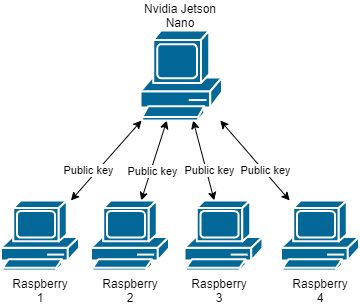
\includegraphics[width=0.5\textwidth]{Figuras/Network_public_key.png}    
    \caption{Intercambio de claves públicas entre los participantes} 
    \label{fig:PublicKeyShare}
\end{figure}

\subsubsection{Entrenamiento}
El entrenamiento es algo que en el protocolo se omite pero que es importante mencionar. Este proceso se lleva a cabo en el dispositivo del participante y conlleva dos tareas:
\begin{itemize}
    \item En primer lugar este participante crea su modelo de inteligencia artificial, lo entrena con los datos que él elija y lo almacena.
    \item En segundo lugar este modelo es cifrado y enviado al servidor. El proceso de cifrado se puede observar en el diagrama \ref{fig:Flow_Encryption} de la sección de securización de las comunicaciones \ref{SegCom}.
\end{itemize} 
\begin{figure}[H]
    \centering
    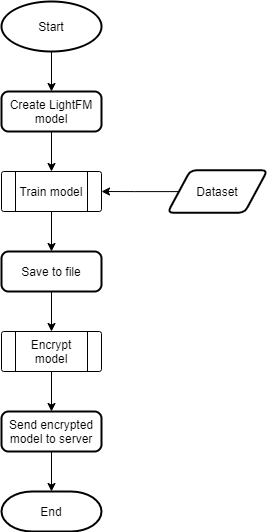
\includegraphics[height=0.6\textheight]{Figuras/flowchart_train.png}    
    \caption{Intercambio de claves públicas entre los participantes} 
    \label{fig:PublicKeyShare}
\end{figure}

\subsubsection{Comunicación con el servidor}
La comunicación con el servidor es un proceso crucial en el que se debe asegurar que los modelos de los participantes lleguen sin modificaciones y sin ser interceptados por ningún atacante. Para securizar este proceso se ha trabajado en una sección donde se explica más a fondo los pasos llevados para conseguir que las comunicaciones sean seguras, sección \ref{SegCom}.
\\ \\
Debido a la seguridad de la red los participantes deberán enviar tanto los modelos cifrados como las claves cifradas como se puede observar en las siguientes imágenes.

\begin{figure}[H]
    \begin{minipage}[t]{0.45\linewidth}  % <---
        \centering
        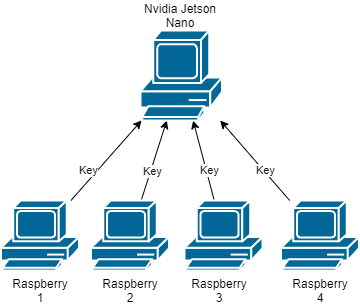
\includegraphics[width=\textwidth]{Figuras/Network_participant_encrypted_key.png}
        \caption{Envío de la clave de cifrado del modelo al servidor de agregación} 
    \end{minipage}
    \hfill
    \begin{minipage}[t]{0.45\linewidth}  % <---
        \centering
        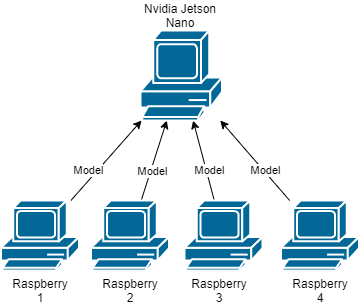
\includegraphics[width=\textwidth]{Figuras/Network_participant_encrypted_model.png}    
        \caption{Envío del modelo cifrado al servidor de agregación} 
    \end{minipage}
\end{figure}

\subsubsection{Agregación de los modelos}
En este proceso como tal no va a ocurrir una agregación de modelos, sino más bien una compartición de conocimiento de forma indirecta mediante el modelo de consenso. Este sistema está explicado con detalle en la sección \ref{Consenso} de este capítulo.
\\ \\
De todas formas para verlo de una forma más sencilla se puede observar el siguiente diagrama \ref{fig:Flow_Agregation} en el cual se muestra el flujo de los datos y de los modelos para ser agregados. El proceso que recorre este diagrama puede ser dividido en 4 partes:
\begin{itemize}
    \item Se reciben los modelos de los participantes (en este caso 4), se descifran siguiendo el diagrama \ref{fig:Flow_Decryption} explicado con detalle en en la sección de securización de las comunicaciones \ref{SegCom} y se guardan los modelos para su posterior utilización.
    \item Una vez se cuente con los modelos descifrados se generan los usuarios sintéticos, después, con el modelo de cada participante se realiza la predicción del ranking para estos usuarios y se almacena para su posterior utilización. 
    \item Mediante el modelo de consenso explicado en el apartado \ref{Consenso} estas predicciones son convertidas a una única predicción por usuario sintético generado. Después la información se almacena para su uso final.
    \item Por último se coge toda la información de los usuarios sintéticos y los rankings consensuados para reentrenar el modelo de cada participante. 
\end{itemize}
\begin{figure}[H]
    \centering
    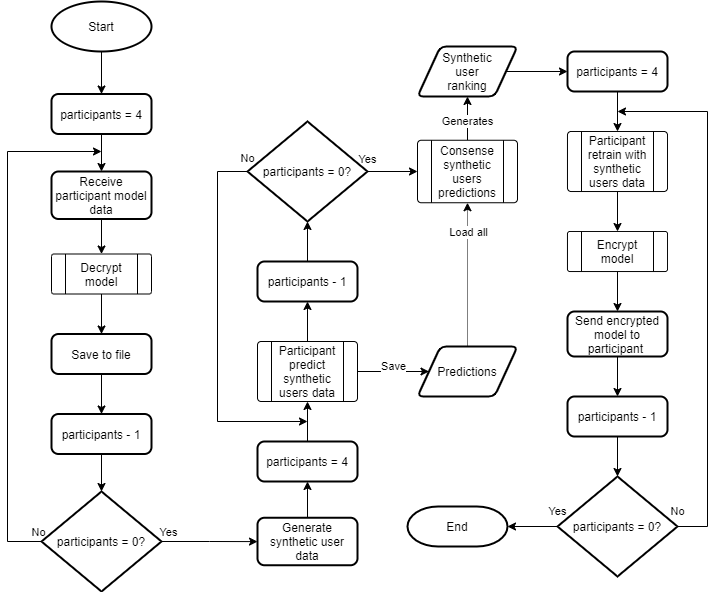
\includegraphics[width=\textwidth]{Figuras/flowchart_agregation.png}    
    \caption{Diagrama del flujo de reentrenado de los modelos} 
    \label{fig:Flow_Agregation}
\end{figure}
\newpage
\subsubsection{Comunicación con los participantes}
La comunicación con los participantes se realiza de la misma forma que los participantes se comunican con el servidor, la única diferencia es que el receptor en este caso son los participantes.
\begin{figure}[H]
    \begin{minipage}[t]{0.45\linewidth}  % <---
        \centering
        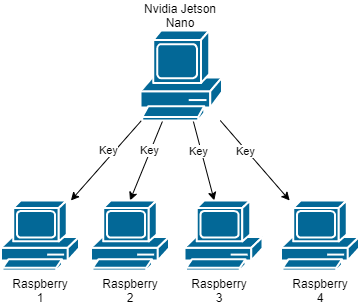
\includegraphics[width=\textwidth]{Figuras/Network_node_encrypted_key.png}
        \caption{Envío de la clave de cifrado del modelo de cada participante a cada participante} 
    \end{minipage}
    \hfill
    \begin{minipage}[t]{0.45\linewidth}  % <---
        \centering
        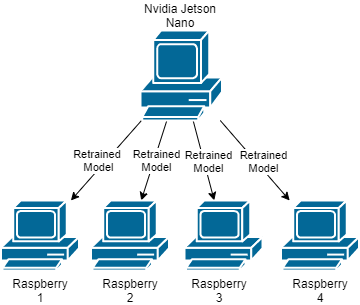
\includegraphics[width=\textwidth]{Figuras/Network_node_encrypted_model.png}    
        \caption{Envío de cada modelo cifrado a su correspondiente dueño} 
    \end{minipage}
\end{figure}
\subsubsection{Comparación de modelos}
En el momento que el modelo llega al participante este tiene que valorar si realmente le supone una mejora o no, para ello como puede verse en el diagrama \ref{fig:Flow_Compare} existen varias fases a llevar a cabo.

En primer lugar, al igual que como con el servidor de agregación se debe descifrar el modelo recibido. Después, compararlo con el modelo del participante, esto se puede hacer tratando de analizar la precisión de las predicciones para varios subconjuntos de datos de test con los que cuente el dispositivo. En resumen, predecir para usuarios existentes su ranking con los dos modelos, y quedarse con el modelo que más acierte.

\begin{figure}[H]
    \centering
    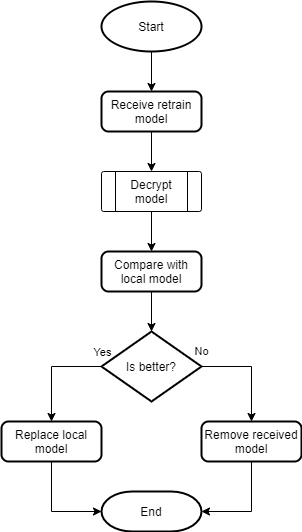
\includegraphics[height=0.6\textheight]{Figuras/flowchart_compare.png}    
    \caption{Diagrama del flujo de la comparación de los modelos} 
    \label{fig:Flow_Compare}
\end{figure}
